\section{CountMax的仿真模拟测试}\label{sec:simulation}
本节中,我们使用仿真环境对CountMax的性能进行评测。

\subsection{仿真环境}
为了使用有限的资源模拟较大规模的网络环境,我们使用C\#语言编写了一个仿真程序,并实现了多种sketch。
通过模拟数据包在交换机之间的传输,并将每个sketch实例分别与仿真环境中的虚拟交换机绑定,可以模拟交换机上的sketch处理数据包的过程。


\subsection{测试指标与基准}\label{subsec:metric}
在仿真模拟测试中,我们采用如下测试指标:
\begin{enumerate}
	\item
    对大流流量的估计的平均误差。在此,我们定义“大流”为网络中按流量排序的前$\alpha$\%的流。
    对每条$f_i$,其相对误差为$|\hat{a}_i-a_i|/a_i$,其中$\hat{a}_i$ 和 $a_i$分别代表流量的估计值和实际值。
    取所有大流的相对误差的平均数为测试指标。
	\item
	sketch的运行时间。让同样的网络流量在同一时刻经过不同的sketch,比较sketch处理这些数据所需的时间。
	尽管仿真环境与实际系统有所区别,但仿真环境下sketch的运行时间仍可以反映出算法之间在时间复杂度上的区别。
%	\item
%	The average number of CPU cycles for processing a packet. Since the running time might be influenced by many external factors (e.g. , JIT compiling, other running processes), we use CPU cycles as another computing overhead metric on the SDN platform \cite{huang2017sketchvisor}. When a packet arrives at a switch, we compute the required number of CPU cycles for processing each packet on average.
	\item
	大流的正确识别比例。如果一个前$\alpha$\%的大流,它的流量估计值也位于前$\alpha$\%中,那么就认为它是被正确识别的。
	我们用正确识别的大流数量和全部的大流数量的比值作为测试指标。
	\item
	最大链路负载率。为了量化重路由的效果,我们收集所有链路的负载,分别除以链路的容量,得到负载率。
	其中的最大值即是“最大链路负载率”。我们采用重路由之后的最大链路负载率和重路由之前的最大链路负载率之比值作为指标。
%and select the maximum link load as the metric. To normalize the metric, for each test case, we choose the maximum link load before rerouting as 1, and compare the relative value.
	\item
	heavy hitter的平均估计误差。\ref{sec:analysis}小节中介绍了heavy hitter的定义。
	“平均估计误差”的定义和第一条指标中的定义相同。
%	\item
%	The maximum number of processed packets per second (pps) that a sketch can support. In the platform, we gradually increase the number of packets for each sketch until the switch's CPU is full-loaded. We use this quantity as the metric.
\end{enumerate}

在之前介绍过的4中sketch中,我们选择CountSketch \cite{charikar2004finding} 和 FSS \cite{homem2010finding}作为对比。
Count-Min\cite{cormode2004improved}和SketchVisor\cite{huang2017sketchvisor}分别因为不能识别大流和计算负载过高而被排除。

\subsection{仿真参数设置}\label{subsec:simulationsetting}

在仿真测试中,我们选择了两种典型且有广泛应用的网络拓扑结构。分别是Fat-tree \cite{al2008scalable}和Spine-Leaf \cite{alizadeh2013data}。
对于其中的Fat-tree拓扑,我们设置为核心层有16个交换机、汇聚层和接入层分别有24个交换机。
Spine-Leaf拓扑则设置为27个“脊”交换机和54个“叶”交换机。其中任意两个叶交换机和脊交换机之间都有一条链路。

为了进行模拟,我们还生成了不同数量的流。
我们使用一份研究院以往的包括约30万条流的网络流量采样,通过插值的方式生成了不同数量的流的流量大小的分布。
由于研究院的网络拓扑和仿真模拟所用的网络拓扑不同,我们还需要对这些流生成路由。
首先对所有的接入交换机和叶交换机赋予一个随机的权重,然后根据权重随机选择交换机作为流的起点和终点。
随后使用最短路径算法计算每条流的初始路由。

在重路由中,我们采用\ref{sec:flowrerouting}小节中描述的贪心法,即优先将最大的流分配到最不拥挤的链路。
如果同时有多条最佳路径,则随机选择其中的一条。

\begin{figure}
    \centering
    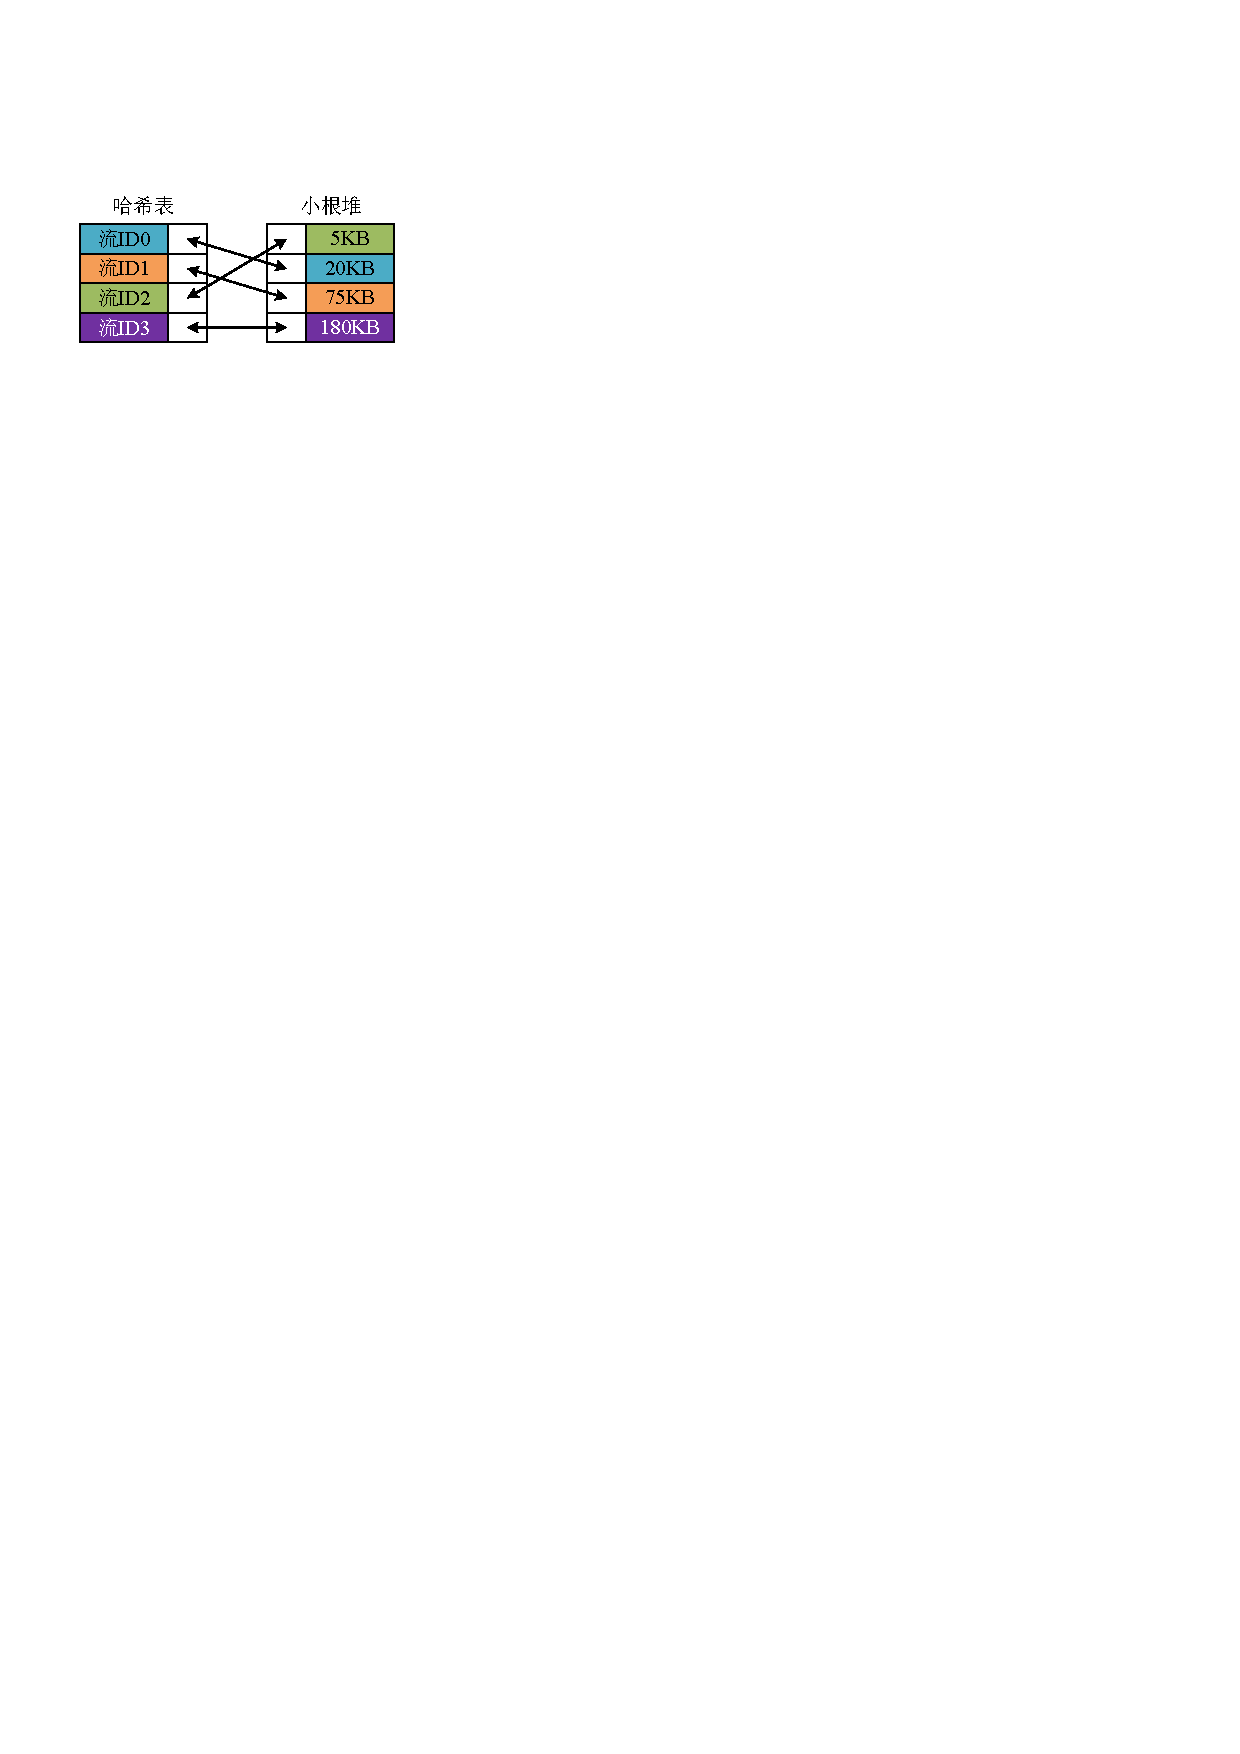
\includegraphics[width=0.6\linewidth]{fig/hashheap.pdf}
    \caption{\textnormal{哈希堆结构的示意图}}
	\label{fig:hashheap}
	\note{图中流0的流量大小为20KB,流1的为75KB,流2的为5KB,流3的为180KB}
 \end{figure}

除此之外,为了让sketch之间的对比更加有意义,我们还对CountSketch和FSS进行了改进。

在第\ref{chap:sketch}章中分析得出CountSketch和FSS在最坏情形下的更新操作的时间复杂度是$O(k)$。
而根据第\ref{chap:countmax}章中的分析,CountMax的更新操作的时间复杂度仅有$O(d)$字节。
由于$k$和$d$之间的数量级相差悬殊,可以预测CountMax的更新速度远远快于CountSketch和FSS。
在此我们通过设计一种空间换时间的方法使得这两种sketch的时间复杂度降为$O(\log{k})$。
图\ref{fig:hashheap}是我们所设计的数据结构的示意图。本文中将其称为“哈希堆”,用来代替CountSketch中的小根堆和FSS中的哈希表。
哈希堆由一个哈希表和一个小根堆组成。其中哈希表的键是流的ID,值是指向小根堆中的元素的指针或索引。
小根堆中的元素包含两个字段,一个是指向哈希表中的一项的指针,另一个则是流量统计的计数器。
哈希表的表项和小根堆的元素总是成对的,并且双方的指针分别指向彼此。每当更新数据的时候两边的指针也会进行更新以保持一致性。
通过这样的方式,哈希堆可以在$O(1)$的时间内测试一个流的ID是否存在,并在$O(\log{k})$的时间内对流量统计值进行更新。

另外,CountMax可以进行协作式部署,我们让CountSketch和FSS也使用类似的策略,进行协作式部署。
在本章中,除特别说明外,所有sketch都是采用如第\ref{sec:coop}小节所述的协作式策略进行部署的。



\subsection{存储占用分析}\label{subsec:memory}

为了进行公平的性能对比,我们希望参与比较的3中sketch使用尽量相同的内存空间。因此首先我们分析这些sketch的存储空间消耗。
表\ref{tbl:datasize}中列出了几种基本数据类型的大小。本文的所有测试中,流的ID都是五元组的形式,其中包含源、目的IP地址和端口,以及协议。
因此,一个五元组的大小是$ (4 + 2 ) \times 2 + 2=14$字节。

\begin{table}[h]
	\centering
    \caption{\textnormal{一些基础数据结构的大小}}
	\begin{tabular}{c|c|c|c|c}
		\hline
		数据类型 & IPv4地址 & 端口/协议号 & 计数器 &指针\\
		\hline
		位数 & 32 & 16 & 64 & 32\\
		\hline
		字节数 & 4 & 2 & 8 & 4\\
		\hline
	\end{tabular}
    \label{tbl:datasize}
\end{table}

图\ref{fig:hashheap}中展示的哈希堆中的一项包含一个哈希表项和一个堆元素,总计包含一个五元组、两个指针和一个计数器。
因此,哈希堆的单位大小是$14+4+4+8=30$个字节。

接下来考虑每种sketch的内存占用。设FSS的bitmap和哈希堆的长度相同,均为$l_{FSS}$;
令$l_{CM}$和$d_{CM}$分别表示CountMax的长度和行数;
CountSketch的bitmap和哈希堆的长度均为$l_{CS}$,bitmap的行数为$d_{CS}$,根据以上的结论,可以计算得出:

\begin{enumerate}
\item 
FSS中,bitmap只有一行,每个格子包含两个计数器,因此FSS的总内存消耗是$(8+8+30)\cdot l_{FSS} = 46\cdot l_{FSS}$字节。
\item CountSketch中的每个格子只有一个计数器,因此内存消耗是$(8\cdot d_{CSketch} + 30)\cdot l_{CSketch}$字节。
\item 对于CountMax,每个格子包含一个14字节的五元组和一个8字节的计数器,因此内存消耗是$22 \cdot d_{CMax}\cdot l_{CMax}$字节。
\end{enumerate}

为了让三种sketch拥有接近的内存消耗,令 $d_{CSketch}=d_{CMax}=2$,$l_{FSS}=l_{CSketch}=l_{CMax}=k$,则三种sketch的内存消耗非常接近并且只取决于$k$。
例如,当$k=1024$的时候,FSS占用$46 \times 1024 = 46$(KB\footnote{kilobyte, 千字节,下同。}),CountSketch占用$(8\times 2 +30)\times 1024 = 46$(KB),CountMax占用$22\times 2\times 1024=44$(KB)。
在接下来的章节中,我们通过改变$k$来控制sketch的存储空间。

\subsection{仿真模拟结果}

\begin{figure}[ht]
	\centering
	\begin{minipage}[t]{0.49\linewidth}
		\centering
		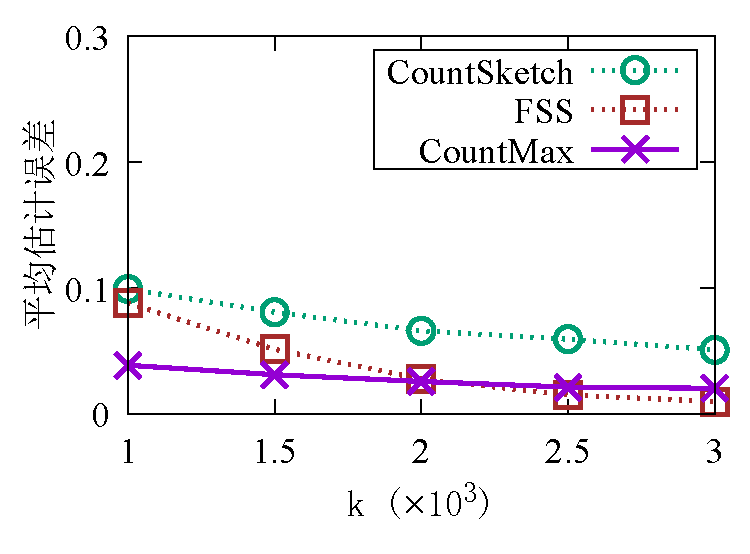
\includegraphics[width=\linewidth]{fig/ft_k_appr_200000_099.pdf}
	\end{minipage}\vspace{-0.6em}%
	\begin{minipage}[t]{0.49\linewidth}
		\centering
		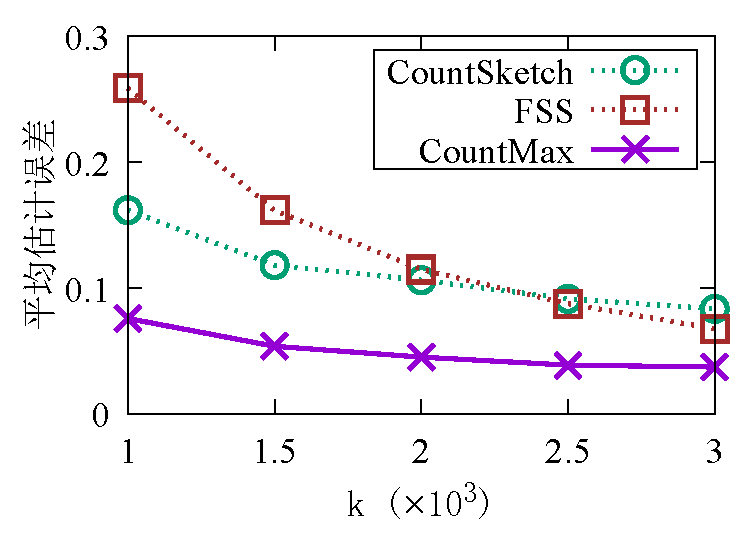
\includegraphics[width=\linewidth]{fig/hy_k_appr_200000_099.pdf}
	\end{minipage}\vspace{-0.6em}%
	\caption{\textnormal{估计误差对比$k$。20万条流,$\alpha = 1\%$。 \textit{左图}: Fat-tree; \textit{右图}: Spine-Leaf。}}
	\label{fig:acc,k,20,1}
\end{figure}

\begin{figure}[ht]
	\centering
	\begin{minipage}[t]{0.49\linewidth}
		\centering
		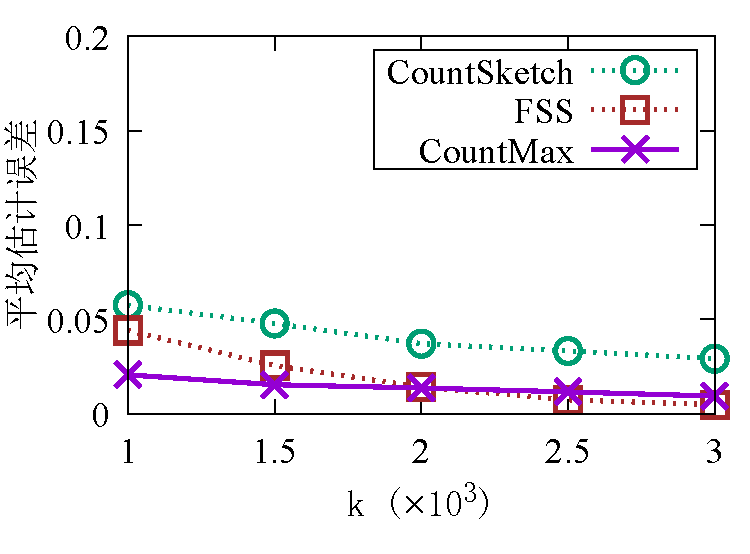
\includegraphics[width=\linewidth]{fig/ft_k_appr_200000_095.pdf}
	\end{minipage}\vspace{-0.6em}%
	\begin{minipage}[t]{0.49\linewidth}
		\centering
		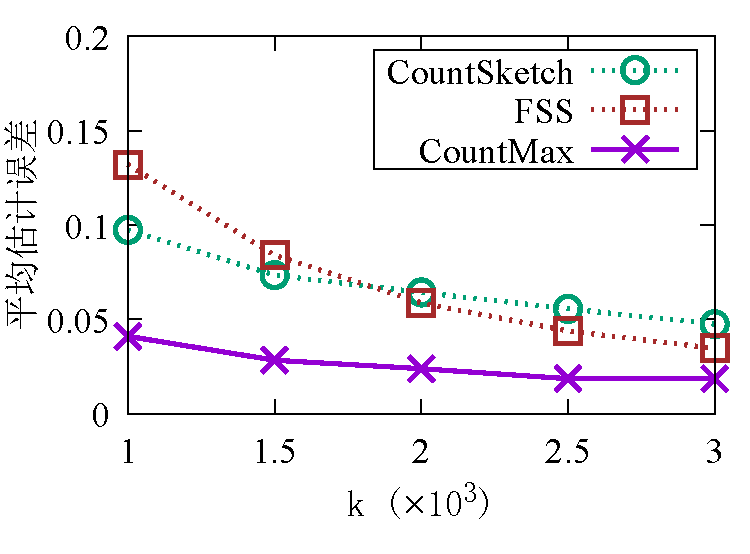
\includegraphics[width=\linewidth]{fig/hy_k_appr_200000_095.pdf}
	\end{minipage} \vspace{-0.6em}%
	\caption{\textnormal{估计误差对比$k$。20万条流,$\alpha = 0.5\%$。 \textit{左图}: Fat-tree; \textit{右图}: Spine-Leaf。}}
	\label{fig:acc,k,20,5}
\end{figure}


\begin{figure}[ht]
	\centering
	\begin{minipage}[t]{0.49\linewidth}
		\centering
		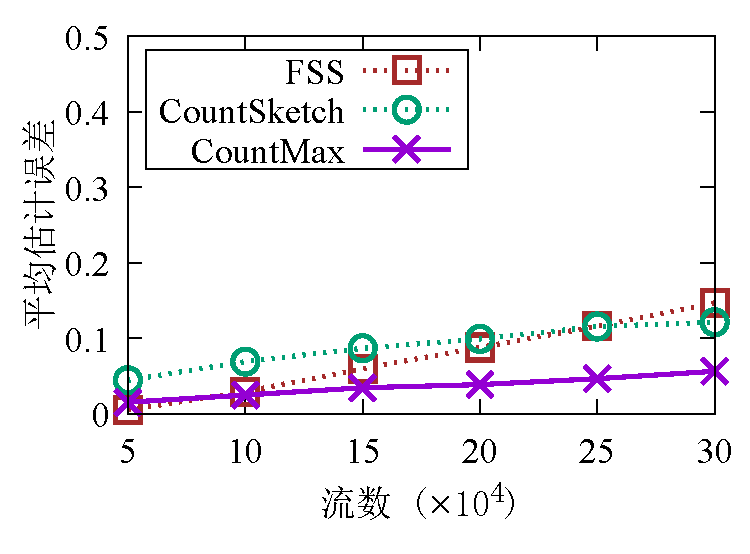
\includegraphics[width=\linewidth]{fig/ft_flow_appr_1000_099.pdf}
	\end{minipage}\vspace{-0.6em}%
	\begin{minipage}[t]{0.49\linewidth}
		\centering
		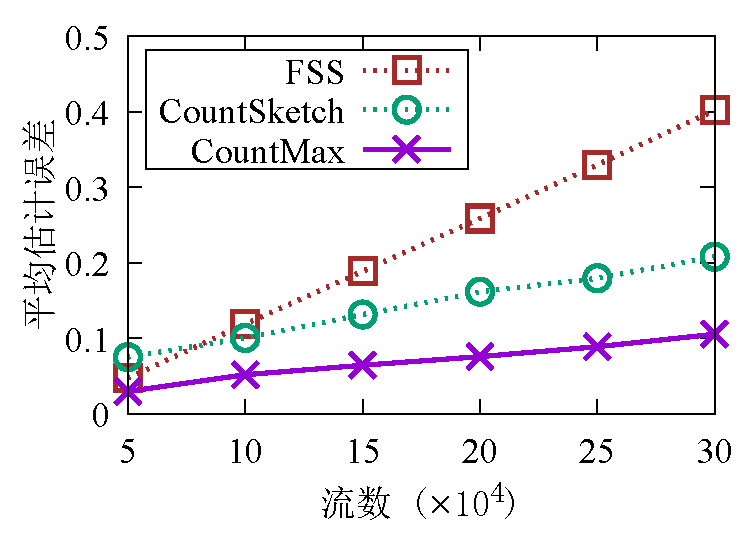
\includegraphics[width=\linewidth]{fig/hy_flow_appr_1000_099.pdf}
	\end{minipage}\vspace{-0.6em}
	\caption{\textnormal{估计误差对比流数。$k=1000$,$\alpha = 1\%$。 \textit{左图}: Fat-tree; \textit{右图}: Spine-Leaf。}}
	\label{fig:acc,f,1000,1}
\end{figure}


\begin{figure}[ht]
	\centering
	\begin{minipage}[t]{0.49\linewidth}
		\centering
		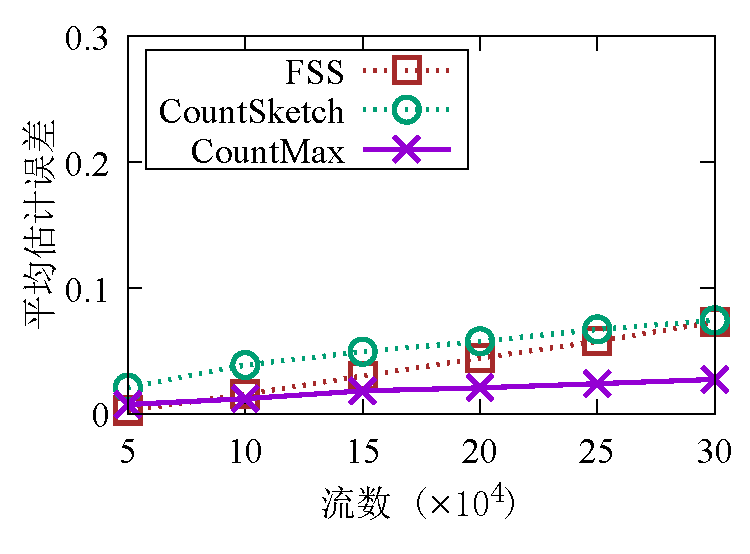
\includegraphics[width=\linewidth]{fig/ft_flow_appr_1000_095.pdf}
	\end{minipage}\vspace{-0.6em}%
	\begin{minipage}[t]{0.49\linewidth}
		\centering
		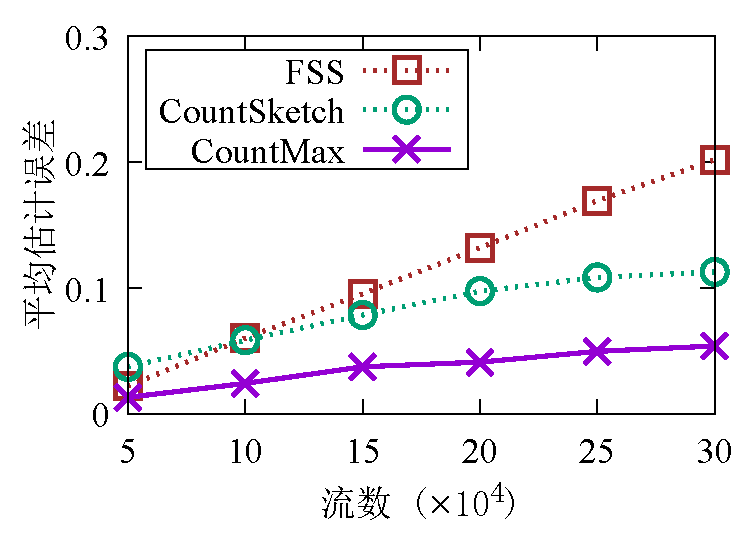
\includegraphics[width=\linewidth]{fig/hy_flow_appr_1000_095.pdf}
	\end{minipage}\vspace{-0.6em}
	\caption{\textnormal{估计误差对比流数。$k=1000$,$\alpha = 0.5\%$。 \textit{左图}: Fat-tree; \textit{右图}: Spine-Leaf。}}
	\label{fig:acc,f,1000,5}
\end{figure}

为了测试不同方向的性能,我们进行了6组测试。第一组是测试平均估计误差随$k$和流数的变化的变化。
我们选取0.5\%和1\%作为两种$\alpha$的取值。
图\ref{fig:acc,k,20,1} 和图 \ref{fig:acc,k,20,5}体现了当网络中有20万条流时,平均估计误差随$k$的变化趋势。
随着$k$的增加,sketch占用的存储空间增加,估计的结果也就更准确。
当$k$比较小的时候,如$k=1000$时,CountSketch和FSS的误差比CountMax大较多。
这是因为CountMax有2行,使用相同的空间可以存放更多的信息,因而减小了误差。
随着$k$增加,CountSketch和FSS的误差大幅下降,变得可以接受;CountMax的误差对$k$不敏感。
总体来讲,和CountSketch以及FSS相比,CountMax将平均估计误差减少了约15\%到30\%。

图\ref{fig:acc,f,1000,1} 和图 \ref{fig:acc,f,1000,5}在$k$固定为1000时,流数的变化如何影响平均估计误差的测试结果。
随着流数的增加,估计误差也随之上升。因为网络中的大流的增加,固定大小的内存空间不足以准确地测量这些流,因而误差增大。
图中显示了FSS相比CountSketch和CountMax,对于流数的变化更敏感。
原因是FSS的bitmap只有一行,因此哈希冲突带来的影响更大。
当流数超过20万时,CountMax的平均估计误差几乎只有CountSketch和FSS的一半。


\begin{figure}[ht]
	\centering
	\begin{minipage}[t]{0.49\linewidth}
		\centering
		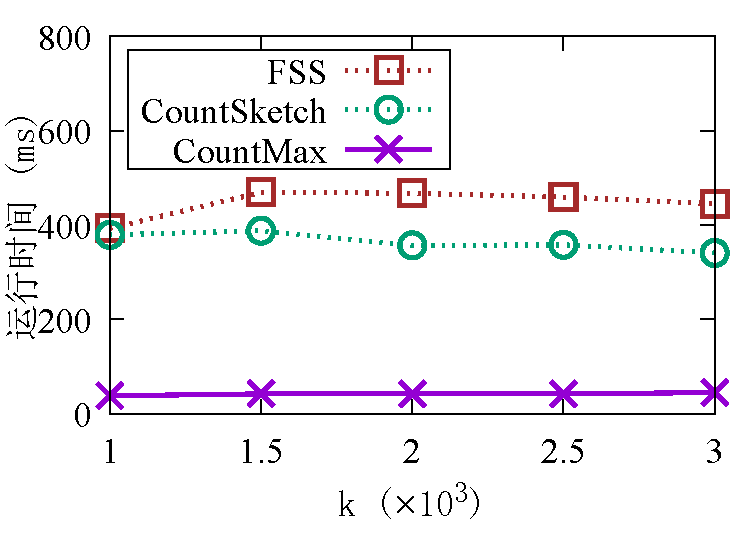
\includegraphics[width=\linewidth]{fig/ft_k_time_200000.pdf}
		%\small{\caption\tiny{Algorithm Execution Time vs. $k$ with 200,000 flows} }
	\end{minipage}\vspace{-0.6em}%
	\begin{minipage}[t]{0.49\linewidth}
		\centering
		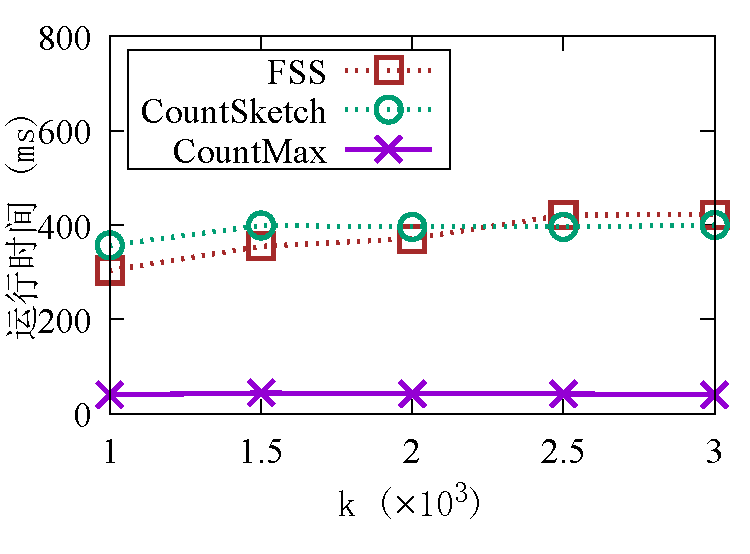
\includegraphics[width=\linewidth]{fig/hy_k_time_200000.pdf}
		%\small{\caption\tiny{Algorithm Execution Time vs. $k$ with 200,000 flows} }
	\end{minipage}\vspace{-0.6em}
	\caption{\textnormal{sketch运行时间与$k$。20万条流。 \textit{左图}: Fat-tree; \textit{右图}: Spine-Leaf。}}
	\label{fig:time,k}
\end{figure}

\begin{figure}[ht]
	\centering
	\begin{minipage}[t]{0.49\linewidth}
		\centering
		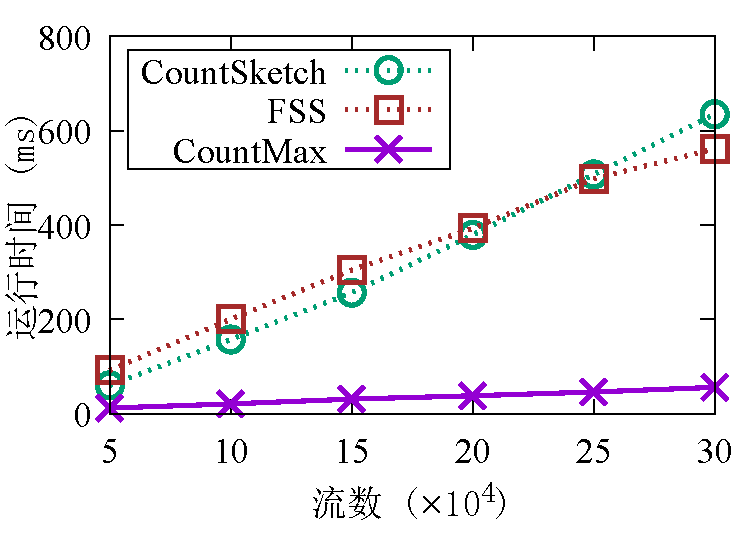
\includegraphics[width=\linewidth]{fig/ft_flow_time_1000.pdf}
		%%\small{\caption{\textnormal{Algorithm Execution Time vs. The number of flows with fixed $k$=1,000}}}
	\end{minipage}\vspace{-0.6em}%
	\begin{minipage}[t]{0.49\linewidth}
		\centering
		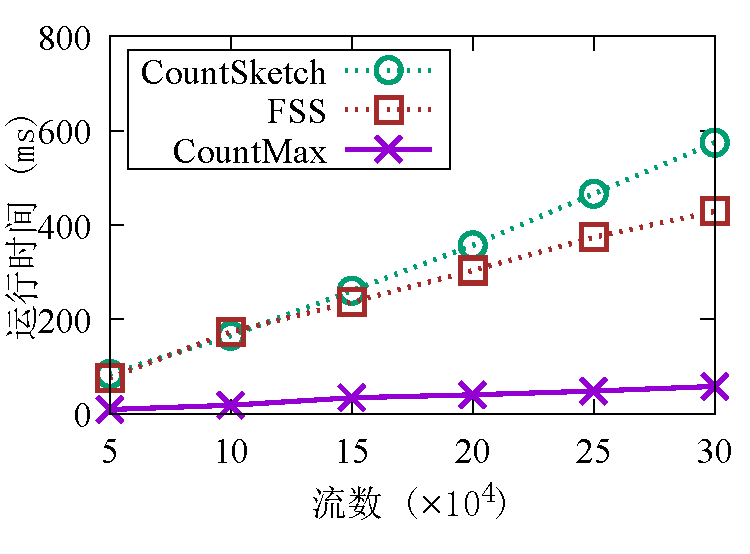
\includegraphics[width=\linewidth]{fig/hy_flow_time_1000.pdf}
		%%\small{\caption{\textnormal{Algorithm Execution Time vs. The number of flows with fixed $k$=1,000}}}
	\end{minipage} \vspace{-0.6em}%
	\caption{\textnormal{sketch运行时间与流数。$k=1000$。 \textit{左图}: Fat-tree; \textit{右图}: Spine-Leaf。}}
	\label{fig:time,f}
\end{figure}

第二组仿真模拟测试的是不同sketch的运行时间。
根据第\ref{chap:sketch}章的理论分析,CountSketch和FSS在最坏情况下的时间复杂度都是$O(\log{k})$。
第\ref{chap:countmax}证明了CountMax在任何情况下的时间复杂度都是$O(1)$。
图 \ref{fig:time,k} 和图 \ref{fig:time,f}印证了这些理论分析。
$k$的变化对CountMax的运行时间几乎没有影响,而CountSketch和FSS的运行时间则随$k$的增长而增长。
原因在于CountMax不需要维护额外的数据结构,从而避免了$O(\log{k})$的操作。
需要强调的是,这组测试是在仿真模拟环境下进行的。实际应用中sketch的实现和仿真器中的实现有较大的不同,因而其计算负载也会和这组实验有所出入。

\begin{figure}[ht]
	\centering
	\begin{minipage}[t]{0.49\linewidth}
		\centering
		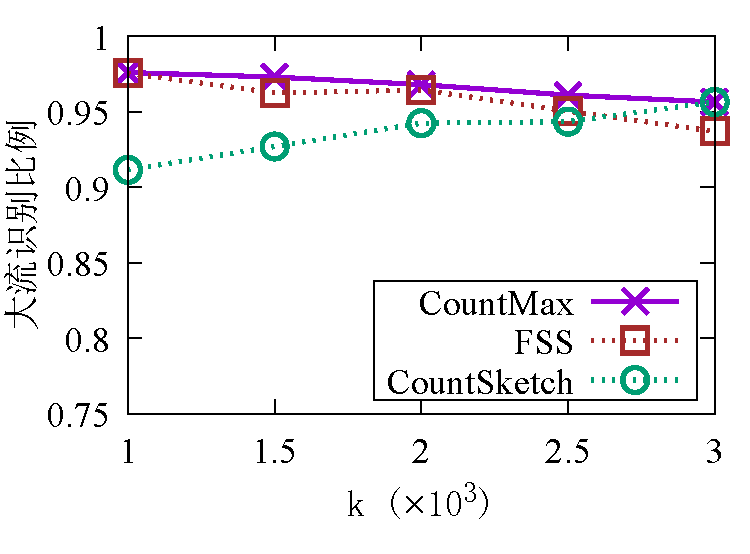
\includegraphics[width=\linewidth]{fig/ft_k_hit_200000.pdf}
		%%%\small{\caption{\textnormal{Elephant Flow Hit Rate vs. $k$ with 200,000 flows, top 0.5\% flows}}}
	\end{minipage}\vspace{-0.6em}%
	\begin{minipage}[t]{0.49\linewidth}
		\centering
		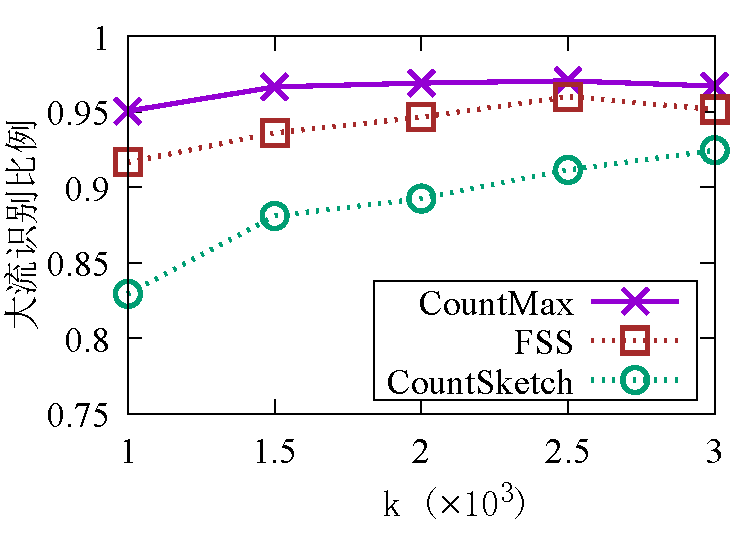
\includegraphics[width=\linewidth]{fig/hy_k_hit_200000.pdf}
		%%%\small{\caption{\textnormal{Elephant Flow Hit Rate vs. $k$ with 200,000 flows, top 0.5\% flows}}}
	\end{minipage} \vspace{-0.6em}%
	\caption{\textnormal{大流识别率与$k$。20万条流。 \textit{左图}: Fat-tree; \textit{右图}: Spine-Leaf。}}
	\label{fig:hit,k,20}
\end{figure}

\begin{figure}[ht]
	\centering
	\begin{minipage}[t]{0.49\linewidth}
		\centering
		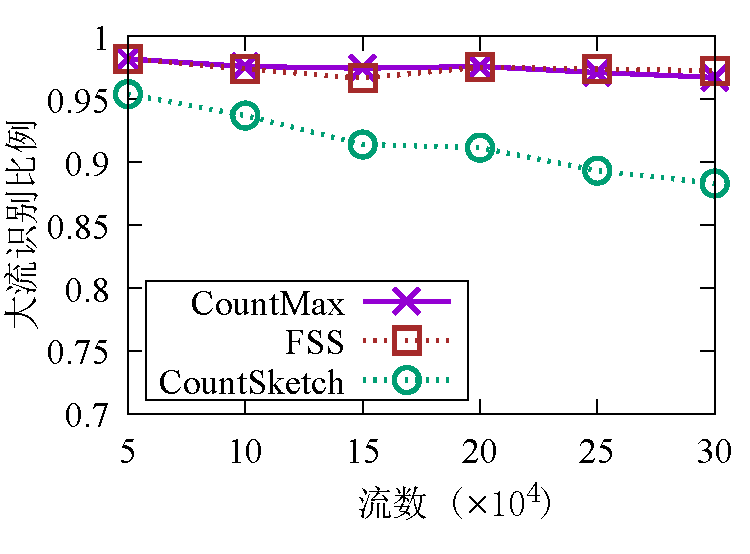
\includegraphics[width=\linewidth]{fig/ft_flow_hit_1000.pdf}
		%%\small{\caption{\textnormal{Elephant Flow Hit Rate vs. The number of flows with fixed $k$=1,000, top 0.5\% flows}}}
	\end{minipage}\vspace{-0.6em}%
	\begin{minipage}[t]{0.49\linewidth}
		\centering
		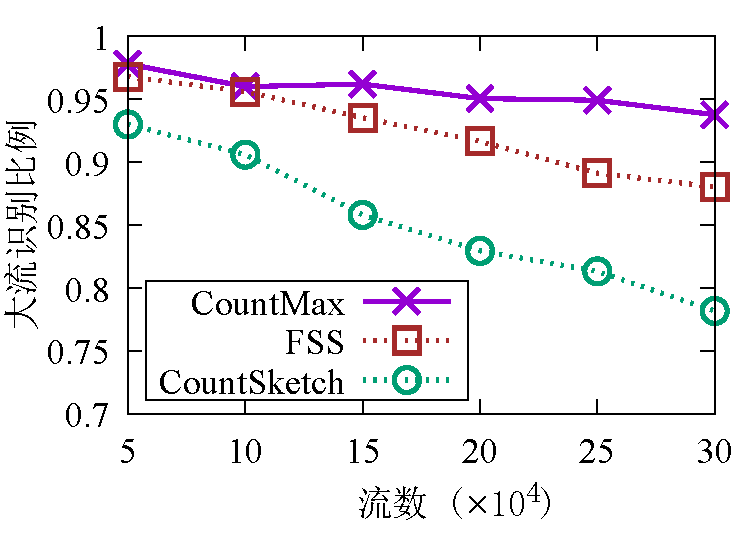
\includegraphics[width=\linewidth]{fig/hy_flow_hit_1000.pdf}
		%%\small{\caption{\textnormal{Elephant Flow Hit Rate vs. The number of flows with fixed $k$=1,000, top 0.5\% flows}}}
	\end{minipage} \vspace{-0.6em}%
	\caption{\textnormal{大流识别率与流数,$k=1000$。 \textit{左图}: Fat-tree; \textit{右图}: Spine-Leaf。}}
	\label{fig:hit,f,1000}
\end{figure}

第三组模拟研究的是$k$与流数如何影响大流识别率。
在图\ref{fig:hit,k,20} 与图 \ref{fig:hit,f,1000}中,当$k$比较小的时候,CountMax可以比CountSketch 和 FSS多识别10\%到20\%的大流。
CountSketch和FSS使用哈希堆存储大流的ID,因此它们能追踪的流的数量和哈希堆的容量相同,也就是$k$。
而CountMax有着独立的两行,因而追踪的流数通常会比$k$更多,从而降低了错误地放过大流的情况。



\begin{figure}[ht]
	\centering
	\begin{minipage}[t]{0.49\linewidth}
		\centering
		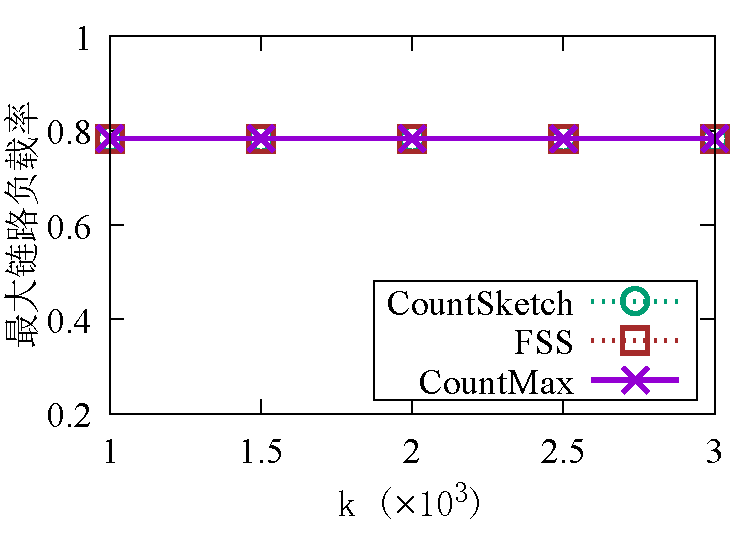
\includegraphics[width=\linewidth]{fig/ft_k_load_200000.pdf}
		%%\small{\caption{\textnormal{Average Link Load vs. $k$ with 200,000 flows} }}
	\end{minipage}\vspace{-0.6em}%
	\begin{minipage}[t]{0.49\linewidth}
		\centering
		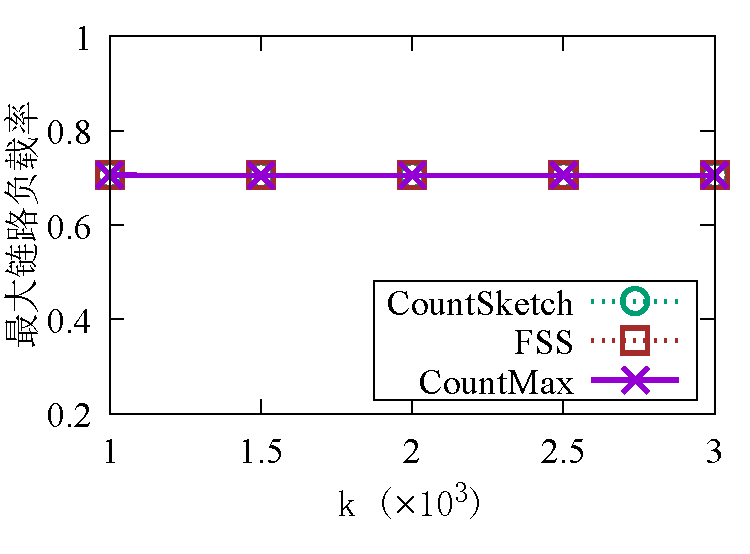
\includegraphics[width=\linewidth]{fig/hy_k_load_200000.pdf}
		%%\small{\caption{\textnormal{Average Link Load vs. $k$ with 200,000 flows} }}
	\end{minipage}\vspace{-0.6em}
	\caption{\textnormal{最大链路负载率与$k$。20万条流。 \textit{左图}: Fat-tree; \textit{右图}: Spine-Leaf。}}
	\label{fig:load,k}
\end{figure}


\begin{figure}[ht]
	\centering
	\begin{minipage}[t]{0.49\linewidth}
		\centering
		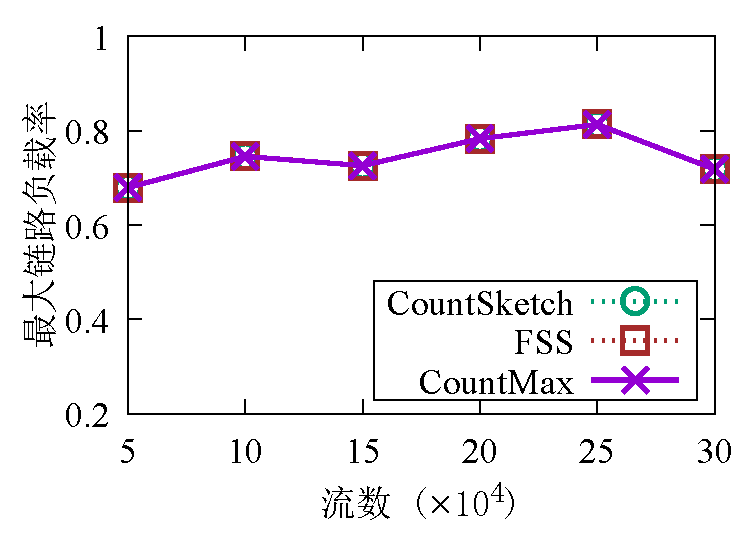
\includegraphics[width=\linewidth]{fig/ft_flow_load_1000.pdf}
		%%\small{\caption{\textnormal{Average Link Load vs. The number of flows with fixed $k$=1,000}}}
	\end{minipage}\vspace{-0.6em}%
	\begin{minipage}[t]{0.49\linewidth}
		\centering
		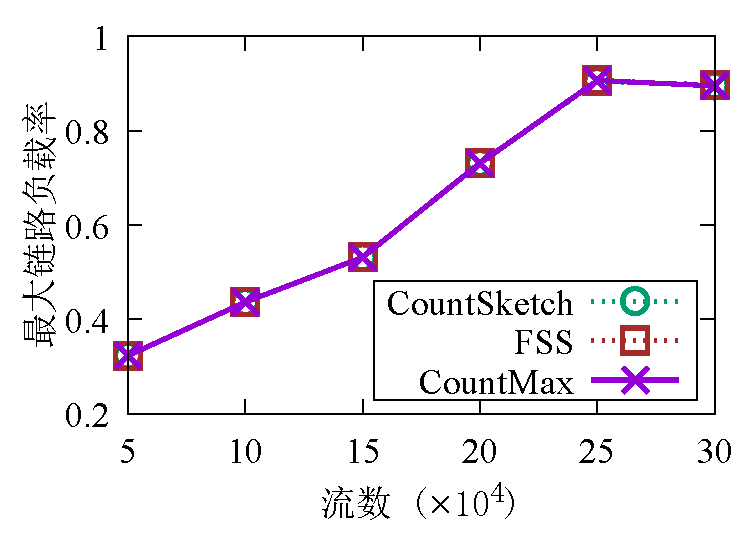
\includegraphics[width=\linewidth]{fig/hy_flow_load_1000.pdf}
		%%\small{\caption{\textnormal{Average Link Load vs. The number of flows with fixed $k$=1,000}}}
	\end{minipage} \vspace{-0.6em}%
	\caption{\textnormal{最大链路负载率与流数。$k=1000$。\textit{左图}: Fat-tree; \textit{右图}: Spine-Leaf。}}
	\label{fig:load,f}
\end{figure}


第四组模拟研究了使用sketch提供的流量统计信息进行重路由的效果。
在所有流量都被处理完成后,仿真平台收集sketch的统计信息,对其中最大的1\%的流使用\ref{sec:flowrerouting}节中提到的贪心法进行重路由。
图\ref{fig:load,k}展示了最大链路负载率和$k$之间的关系。
从第一组测试的结果得知,即使$k$较小,各种sketch的平均估计误差也没有太大,而且重路由对于估计误差的容忍度较高,因此实际上增加$k$并没有使得重路由的性能更好。
图\ref{fig:load,f}显示的是流数对于最大链路负载率的影响。
网络中的流越多,sketch能追踪的大流的比例就越少,因而链路负载率就更高。
从这一组模拟可以看出,三种sketch在用于重路由时,有着几乎完全相同的性能。

\begin{figure}[ht]
	\centering
	\begin{minipage}[t]{0.49\linewidth}
		\centering
		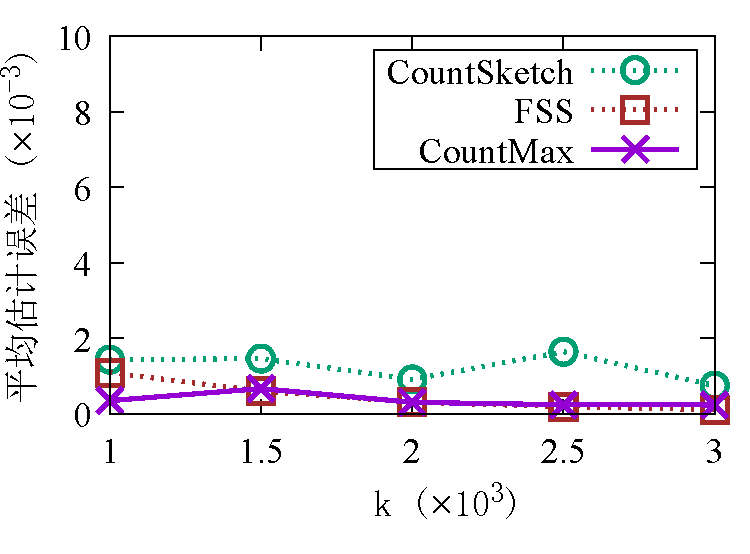
\includegraphics[width=\linewidth]{fig/ft_k_hh_1000.pdf}
	\end{minipage}\vspace{-0.6em}%
	\begin{minipage}[t]{0.49\linewidth}
		\centering
		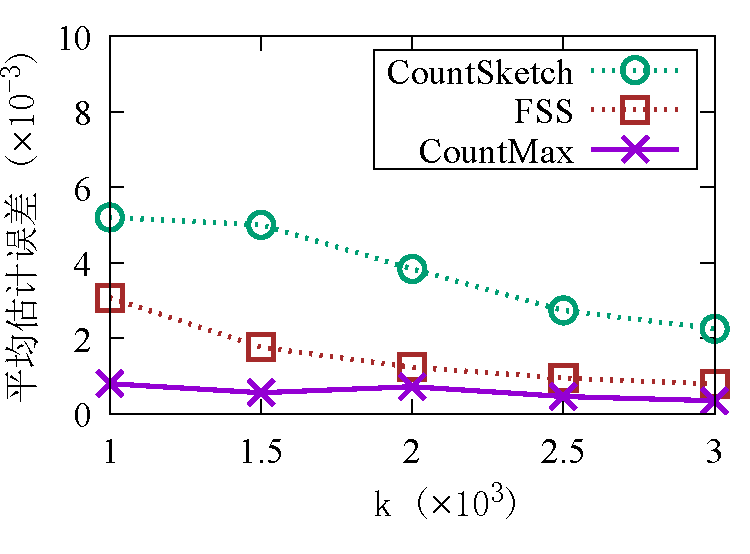
\includegraphics[width=\linewidth]{fig/hy_k_hh_1000.pdf}
	\end{minipage}\vspace{-0.6em}%
	\caption{\textnormal{heavy hitter估计误差与$k$。$\delta=10^{-3}$。 \textit{左图}: Fat-tree; \textit{右图}: Spine-Leaf。}}
	\label{fig:hh,k,1000}
\end{figure}

\begin{figure}[ht]
	\centering
	\begin{minipage}[t]{0.49\linewidth}
		\centering
		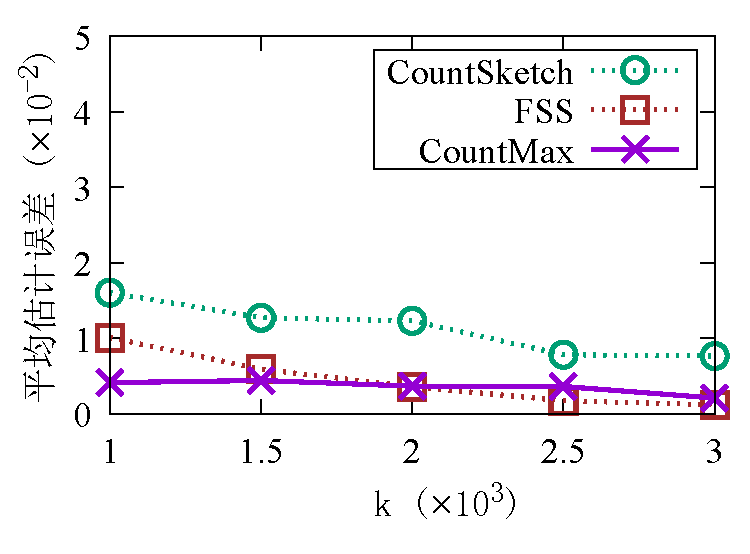
\includegraphics[width=\linewidth]{fig/ft_k_hh_10000.pdf}
	\end{minipage}\vspace{-0.6em}%
	\begin{minipage}[t]{0.49\linewidth}
		\centering
		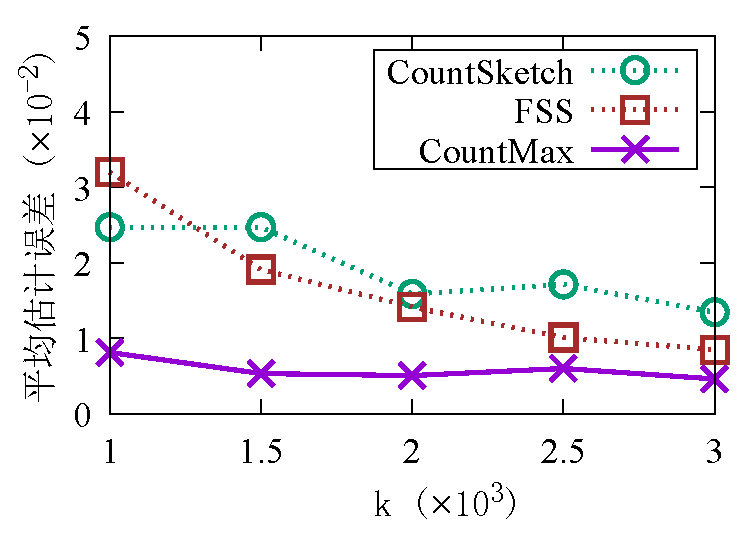
\includegraphics[width=\linewidth]{fig/hy_k_hh_10000.pdf}
	\end{minipage}\vspace{-0.6em}%
	\caption{\textnormal{heavy hitter估计误差与$k$。$\delta=10^{-4}$。 \textit{左图}: Fat-tree; \textit{右图}: Spine-Leaf。}}
	\label{fig:hh,k,10000}
\end{figure}

第5组模拟研究的是heavy hitter的平均估计误差与$k$的关系。在这组模拟中,我们选择$\delta$为$10^{-3}$ 和 $10^{-4}$。
从图\ref{fig:hh,k,1000}到图\ref{fig:hh,k,10000}当中,我们发现,当$\delta =10^{-3}$ 时,三种sketch对heavy hitter的估计都很准确。
这是因为heavy hitter的数目通常很少。如在这次模拟使用的流中,总共只有几十个$10^{-3}$-heavy hitter。
当$\delta = 10^{-4}$时,CountMax的误差略小于CountSketch和FSS。
总而言之,在测量heavy hitter上,CountMax的性能略优于CountSketch和FSS。


\begin{figure}[ht]
	\centering
	\begin{minipage}[t]{0.49\linewidth}
		\centering
		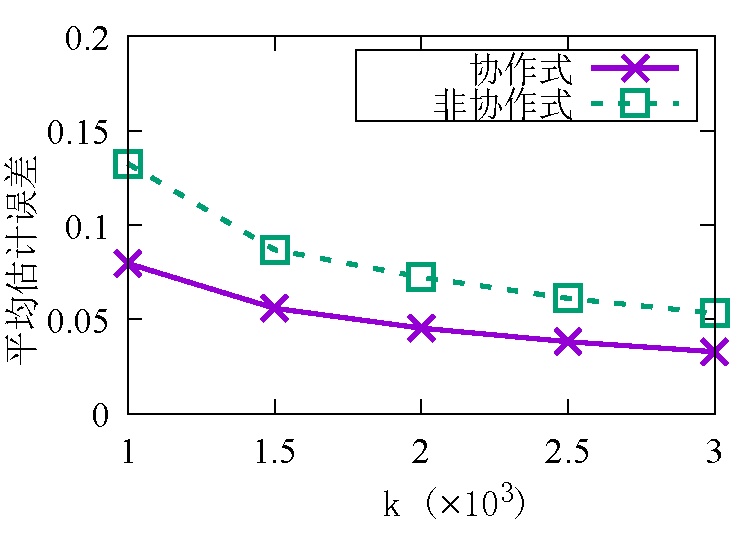
\includegraphics[width=\linewidth]{fig/half_eg_099_k.pdf}
	\end{minipage}\vspace{-0.6em}%
	\begin{minipage}[t]{0.49\linewidth}
		\centering
		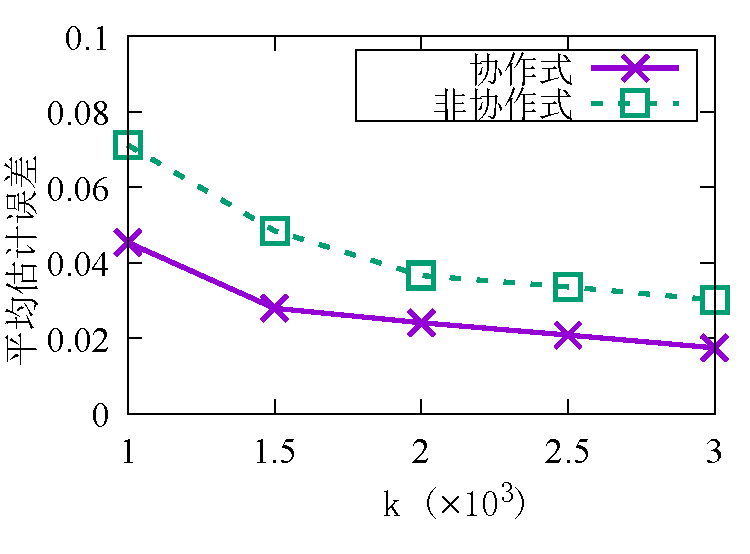
\includegraphics[width=\linewidth]{fig/half_eg_095_k.pdf}
	\end{minipage}\vspace{-0.6em}%
	\caption{\textnormal{平均估计误差与$k$。20万条流,Spine-Leaf。 \textit{左图}: top 1\%; \textit{右图}: top 0.5\%.}}
	\label{fig:coop,acc,k}
\end{figure}

\begin{figure}[ht]
	\centering
	\begin{minipage}[t]{0.49\linewidth}
		\centering
		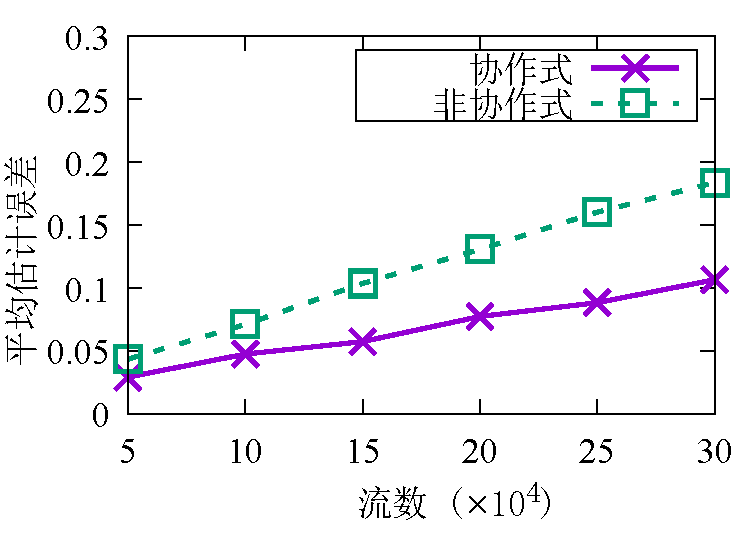
\includegraphics[width=\linewidth]{fig/half_eg_099_flow.pdf}
	\end{minipage}\vspace{-0.6em}%
	\begin{minipage}[t]{0.49\linewidth}
		\centering
		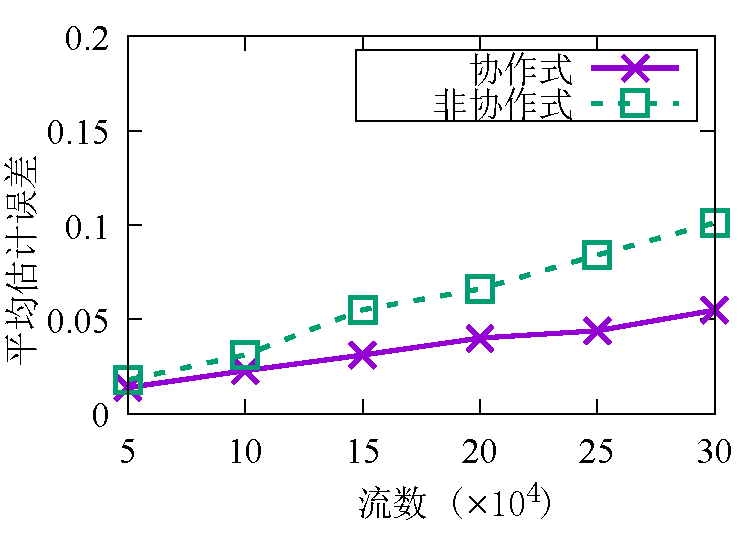
\includegraphics[width=\linewidth]{fig/half_eg_095_flow.pdf}
	\end{minipage}\vspace{-0.6em}%
	\caption{\textnormal{平均估计误差与流数。$k=1000$,Spine-Leaf。 \textit{左图}: top 1\%; \textit{右图}: top 0.5\%.}}
	\label{fig:coop,acc,flow}
\end{figure}

\begin{figure}[ht]
	\centering
	\begin{minipage}[t]{0.48\linewidth}		
		%\begin{figure}[ht]
		\centering
		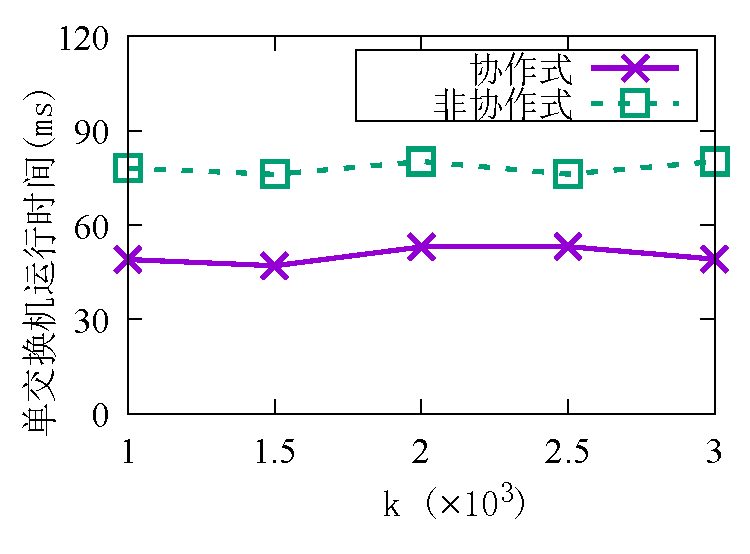
\includegraphics[width=\linewidth]{fig/half_eg_time_k.pdf}
		\caption{\textnormal{最大运行时间与$k$。20万条流,Spine-Leaf。}}
		\label{fig:coop,time,k}
		%\end{figure}
	\end{minipage}\vspace{-0.6em}\hspace{0.4em}
	\begin{minipage}[t]{0.48\linewidth}
		\centering
		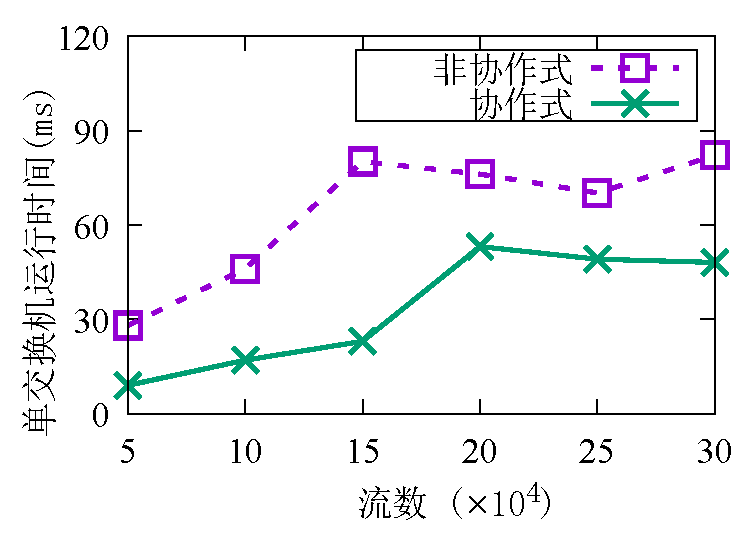
\includegraphics[width=\linewidth]{fig/half_eg_time_flow.pdf}
		\caption{\textnormal{最大运行时间与流数。$k=1000$,Spine-Leaf。}}
		\label{fig:coop,time,flow}
	\end{minipage}\vspace{-0.6em}
\end{figure}

最后一组模拟是在协作式CountMax和非协作式CountMax之间进行对比。
我们选择了Spine-Leaf的拓扑,将其中的叶交换机等分为两组。
其中一组的交换机只向外发送流量,而另一组只接收流量。这是一种极端情况,不过现实中的服务器集群之间同步数据时会出现类似的情况。
从图\ref{fig:coop,acc,k}到图\ref{fig:coop,acc,flow}当中,我们可以看到,相比于非协作式的CountMax,协作式CountMax的平均估计误差减少了30\%到50\%左右。
这是因为协作式CountMax通过将流分配给两端的交换机,避免了一条流被重复测量,减少了哈希冲突从而提高了内存空间的利用率。
图\ref{fig:coop,time,k}到\ref{fig:coop,time,flow}显示了网络中单个交换机的最大负载。
得益于测量任务的分配,协作式CountMax将这一指标降低了30\%到40\%,节约了更多的计算资源。

依据这些模拟结果,我们可以得出以下结论。第一,CountMax有着比CountSketch和FSS更低的计算负载。随着$k$的增加,CountMax的运行时间最低只有CountSketch和FSS的十分之一。
第二,CountMax的估计精度更高。具体而言,CountMax的平均估计误差比CountSketch和FSS低约20\%。
第三,CountMax在重路由的应用中可以达到和CountSketch和FSS相同的性能。
最后,协作式CountMax和非协作式相比,最多可以降低40\%左右的误差和计算负载。





